\documentclass{article}
\usepackage[utf8]{inputenc}
\usepackage[spanish]{babel}
\usepackage{graphicx}

\title{Informe de Sistema Experto de Diagnóstico Médico}
\author{Marco Morales}
\date{04/05/2024}

\begin{document}

\maketitle

\section{Introducción}

Este informe presenta el diseño y la implementación de un sistema experto dedicado al diagnóstico médico. La creciente necesidad de diagnóstico correcto basándonos en el conocimiento experto me ha motivado la creación de este sistema. 
Su finalidad es diagnosticar la enfermedad sobre la base de los síntomas, proporcionando información del tratamiento requerido.

\section{Descripción del Sistema Experto}

El sistema experto está diseñado para diagnosticar la enfermedad y su tratamiento luego de la respuesta de diferentes preguntas. Utiliza la base de conocimiento de médicos expertos y técnicas de inferencia para proporcionar la información requerida para el diagnóstico. La interacción con el usuario se maneja a través de la línea de comandos.

\section{Resultados}

Se presenta las capturas de pantalla de la ejecución del sistema experto.

\begin{figure}[h!]
  \centering
  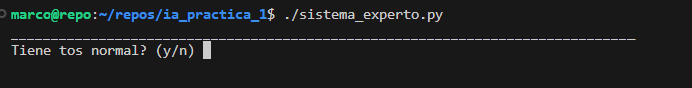
\includegraphics[width=0.8\textwidth]{1.png}
  \caption{Interfaz de usuario del sistema experto con la entrada de síntomas del paciente.}
\end{figure}

\begin{figure}[h!]
  \centering
  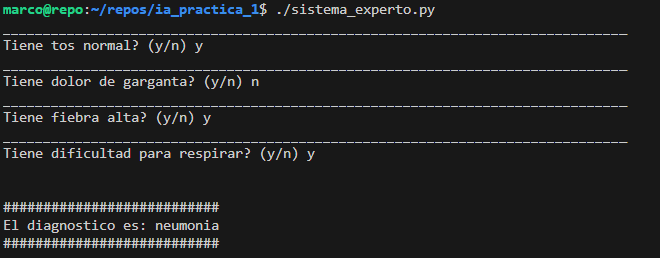
\includegraphics[width=0.8\textwidth]{2.png}
  \caption{Resultado de diagnóstico proporcionado por el sistema experto.}
\end{figure}

\begin{figure}[h!]
  \centering
  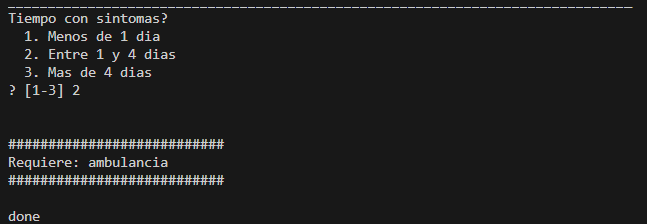
\includegraphics[width=0.8\textwidth]{3.png}
  \caption{Resultado de recomendación de tratamiento proporcionado por el sistema experto.}
\end{figure}
\clearpage
\section{Conclusiones}

El sistema experto demostró ser una herramienta valiosa en diagnóstico de enfermedades. A través de la implementación de un sistema experto basado en reglas y la estrategia de backward chaining, fue posible lograr inferir el diagnóstico correcto.   No obstante, se identificaron áreas de mejora, como poder proporcionar más de un diagnóstico si fuera necesario, que se abordarán en futuros trabajos.

\end{document}